\documentclass[11pt,letterpaper,boxed]{hmcpset}
\usepackage{fullpage}
\setlength{\parskip}{6pt}
\setlength{\parindent}{0pt}
\usepackage[margin=1in]{geometry}
\usepackage{graphicx}
\usepackage{enumerate}
\usepackage{marvosym}
\usepackage{amssymb}
\usepackage{wasysym}
\usepackage{gensymb}
\usepackage{mathrsfs}
\usepackage{scrextend}
\usepackage{mathtools}
\usepackage{pgfplots}
\usepackage{caption}
\usepackage{xspace}
\usepackage[colorlinks]{hyperref}

\makeatletter
\renewcommand*\env@matrix[1][*\c@MaxMatrixCols c]{%
   \hskip -\arraycolsep
   \let\@ifnextchar\new@ifnextchar
   \array{#1}}
\makeatother

% --- style --- %
\renewcommand{\labelenumi}{{ (\alph{enumi})}}
\newcommand{\sand}{\quad \mbox{ and } \quad}
%\newcommand{\ds}{\displaystyle}
\allowdisplaybreaks

% --- making \xi look less awful --- %
\DeclareSymbolFont{CMletters}{OML}{cmm}{m}{it}
\DeclareMathSymbol{\xi}{\mathord}{CMletters}{"18}

% --- math --- %
\newcommand{\Z}{\mathbb{Z}}
\newcommand{\R}{\mathbb{R}}
\newcommand{\C}{\mathbb{C}}
\newcommand{\Q}{\mathbb{Q}}


\newcommand{\Lt}[1]{\mathcal{L}\crb{#1}}
\newcommand{\ilt}[1]{\mathcal{L}^{-1}\crb{#1}}

\newcommand{\pn}[1]{\left( #1 \right)}
\newcommand{\sqb}[1]{\left[ #1 \right]}
\newcommand{\crb}[1]{\left\{ #1 \right\}}
\newcommand{\lra}[1]{\left\langle #1 \right\rangle}
\newcommand{\magn}[1]{\left\lVert #1 \right\rVert}

\newcommand{\pdr}[2]{\frac{\partial #1}{\partial #2}}
\newcommand{\im}[1]{\text{im}\pn{#1}}
\newcommand{\m}[1]{\Z/#1\Z}

\newcommand{\VEC}[1]{\ensuremath{\mathbf{#1}}\xspace}
\DeclareMathOperator{\proj}{proj}
\newcommand{\vectorproj}[2][]{\proj_{\VEC{#1}}\VEC{#2}}

\newenvironment{amatrix}[1]{%
  \left(\begin{array}{@{}*{#1}{c}|c@{}}
}{%
  \end{array}\right)
}

\makeatletter
\renewcommand*\env@matrix[1][*\c@MaxMatrixCols c]{%
  \hskip -\arraycolsep
  \let\@ifnextchar\new@ifnextchar
  \array{#1}}
\makeatother

\newcommand{\spn}[1]{\text{span}\pn{#1}}

\newcommand*\Heq{\ensuremath{\overset{\kern2pt H}{=}}}

\name{Box \#$\rule{1cm}{0.15mm}$}
\class{Math 60 Section 1}
\assignment{Homework 6}
\duedate{22 May 2018}

\begin{document}

%\begin{center}
\noindent\textbf{Collaborators:} 
%\end{center} 

%\problemlist{}

\begin{problem}[Colley 3.4 \#4]
Calculate the divergence of the vector field
\[
	\mathbf{F} = z\cos{e^{y^2}}\mathbf{i} + x\sqrt{z^2+1}\mathbf{j} + e^{2y}\sin{3x}\mathbf{k}.
\]
\end{problem}

\begin{solution}
\vfill
\end{solution}
\newpage

\begin{problem}[Colley 3.4 \#7]
Find the curl of the vector field
\[
	\mathbf{F} = x^2\mathbf{i} - xe^y\mathbf{j} + 2xyz\mathbf{k}.
\]
\end{problem}

\begin{solution}
\vfill
\end{solution}
\newpage

\begin{problem}[Colley 3.4 \#12]
\begin{enumerate}
\item Consider the vector field
\[
	\mathbf{F} = x\mathbf{i} + y\mathbf{j} + z\mathbf{k}
\]
and its curl. Sketch the vector field and use your picture to explain geometrically why the curl is what you calculated.
\item Use geometry to determine $\nabla \times \mathbf{F}$ where
\[
	\mathbf{F} = \frac{\pn{x\mathbf{i} + y\mathbf{j} + z\mathbf{k}}}{\sqrt{x^2+y^2+z^2}}.
\]
\item for $\mathbf{F}$ in part (b), verify your intuition by explicitly computing $\nabla \times \mathbf{F}$.
\end{enumerate}
\end{problem}

\begin{solution}
\vfill
\end{solution}
\newpage

\begin{problem}[Colley 3.4 \#13]
Can you tell in what portions of $\R^2$, the following vector fields have positive divergence? Negative divergence?\\

\begin{center}
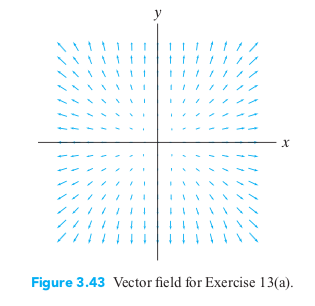
\includegraphics[scale=0.55]{grapA.png} \qquad
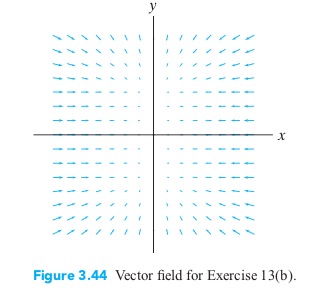
\includegraphics[scale=0.55]{grapB.png}

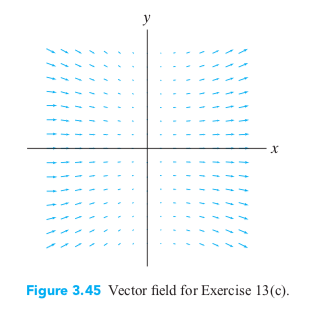
\includegraphics[scale=0.55]{grapC.png} \qquad
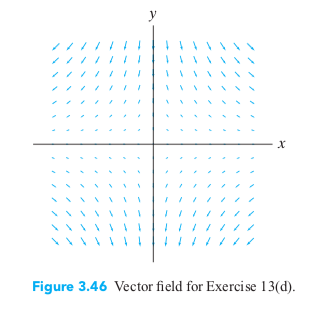
\includegraphics[scale=0.55]{grapD.png}
\end{center}
\end{problem}

\begin{solution}
\vfill
\end{solution}
\newpage

\begin{problem}[Colley 3.4 \#16]
Prove Theorem 4.4: Let $\mathbf{F}: X\subseteq \R^3\rightarrow \R^3$ be a vector field of class $C^2$. Then 
\[
	\text{div (curl }\mathbf{F}) = 0.
\]
That is, curl $\mathbf{F}$ is an
incompressible vector field.
\end{problem}

\begin{solution}
\vfill
\end{solution}
\newpage

\begin{problem}[Colley 3.4 \#23]
Establish
\[
	\nabla \cdot (f\mathbf{F}) = f\nabla \cdot \mathbf{F} + \mathbf{F}\cdot \nabla f.
\]
(You may assume that any functions and vector fields are appropriately differentiable.)
\end{problem}

\begin{solution}
\vfill
\end{solution}


\end{document}